\documentclass{vkr}
\usepackage[english, russian]{babel} % переносы
\usepackage{graphicx} % для вставки картинок
\graphicspath{{images/}} % путь к изображениям
\usepackage[hidelinks]{hyperref}
\usepackage{float} % определяет метод H для рисунка с переносом на следующую страницу, ели не помещается
\usepackage{pdflscape}
\addto{\captionsrussian}{\renewcommand{\refname}{СПИСОК ИСПОЛЬЗОВАННЫХ ИСТОЧНИКОВ}}
\usepackage{xltabular} % для вставки таблиц
\usepackage{makecell}
\renewcommand\theadfont{} % шрифт в /thead
\usepackage{array} % для определения новых типов столбцов таблиц
\newcolumntype{T}{>{\centering\arraybackslash}X} % новый тип столбца T - автоматическая ширина столбца с выравниванием по центру
\newcolumntype{R}{>{\raggedleft\arraybackslash}X} % новый тип столбца R - автоматическая ширина столбца с выравниванием по правому краю
\newcolumntype{C}[1]{>{\centering\let\newline\\\arraybackslash\hspace{0pt}}m{#1}} % новый тип столбца C - фиксированная ширина столбца с выравниванием по центру
\newcolumntype{r}[1]{>{\raggedleft\arraybackslash}p{#1}} % новый тип столбца r - фиксированная ширина столбца с выравниванием по правому краю
\newcommand{\centrow}{\centering\arraybackslash} % командой \centrow можно центрировать одну ячейку (заголовок) в столбце типа X или p, оставив в оcтальных ячейках другой тип выравнивания
\newcommand{\finishhead}{\endhead\hline\endlastfoot}
\newcommand{\continuecaption}[1]{\captionsetup{labelformat=empty} \caption[]{#1}\\ \hline }
\usepackage{etoolbox}
\AtBeginEnvironment{xltabular}{\refstepcounter{tablecnt}} % подсчет таблиц xltabular, обычные таблицы подсчитываются в классе

\usepackage[tableposition=top]{caption} % подпись таблицы вверху
\captionsetup{strut=off}
\setlength{\intextsep}{0pt} % Vertical space above & below [h] floats
\setlength{\textfloatsep}{0pt} % Vertical space below (above) [t] ([b]) floats
\DeclareCaptionLabelFormat{gostfigure}{Рисунок #2} %подпись рисунка
\DeclareCaptionLabelFormat{gosttable}{Таблица #2} %подпись таблицы
\DeclareCaptionLabelSeparator{gost}{~--~} %разделитель в рисунках и таблицах
\captionsetup{labelsep=gost}
\captionsetup[figure]{aboveskip=10pt,belowskip=4mm,justification=centering,labelformat=gostfigure} % настройка подписи рисунка
\captionsetup[table]{font={stretch=1.41},skip=0pt,belowskip=0pt,aboveskip=8.5pt,singlelinecheck=off,labelformat=gosttable} % настройка подписи таблицы

\setlength{\LTpre}{8mm} % отступ сверху таблицы
\setlength{\LTpost}{6mm} % отступ снизу таблицы

\usepackage{enumitem}
\setlist{nolistsep,wide=\parindent,itemindent=*} % отступы вокруг списков, выравнивание с учетом разделителя

\usepackage{color} %% это для отображения цвета в коде
\usepackage{listings} %% листинги кода
\setmonofont[Scale=0.7]{Verdana} % моноширный шрифт для листинга

\definecolor{codegreen}{rgb}{0,0.6,0}
\definecolor{codegray}{rgb}{0.5,0.5,0.5}
\definecolor{codepurple}{rgb}{0.58,0,0.82}

\lstset{ %
language=C,                 % выбор языка для подсветки (здесь это С)
numbers=left,               % где поставить нумерацию строк (слева\справа)
numberstyle=\tiny,           % размер шрифта для номеров строк
stepnumber=1,                   % размер шага между двумя номерами строк
numbersep=5pt,                % как далеко отстоят номера строк от подсвечиваемого кода
commentstyle=\color{codegreen},
keywordstyle=\color{magenta},
numberstyle=\tiny\color{codegray},
stringstyle=\color{codepurple},
basicstyle=\linespread{0.95}\ttfamily,
backgroundcolor=\color{white}, % цвет фона подсветки - используем \usepackage{color}
showspaces=false,            % показывать или нет пробелы специальными отступами
showstringspaces=false,      % показывать или нет пробелы в строках
showtabs=false,             % показывать или нет табуляцию в строках
frame=single,              % рисовать рамку вокруг кода
tabsize=2,                 % размер табуляции по умолчанию равен 2 пробелам
captionpos=t,              % позиция заголовка вверху [t] или внизу [b] 
breaklines=true,           % автоматически переносить строки (да\нет)
breakatwhitespace=false, % переносить строки только если есть пробел
escapeinside={\%*}{*)}   % если нужно добавить комментарии в коде
}

\makeatletter % чтобы допускались русские комментарии в листингах
\lst@InputCatcodes
\def\lst@DefEC{%
 \lst@CCECUse \lst@ProcessLetter
  ^^80^^81^^82^^83^^84^^85^^86^^87^^88^^89^^8a^^8b^^8c^^8d^^8e^^8f%
  ^^90^^91^^92^^93^^94^^95^^96^^97^^98^^99^^9a^^9b^^9c^^9d^^9e^^9f%
  ^^a0^^a1^^a2^^a3^^a4^^a5^^a6^^a7^^a8^^a9^^aa^^ab^^ac^^ad^^ae^^af%
  ^^b0^^b1^^b2^^b3^^b4^^b5^^b6^^b7^^b8^^b9^^ba^^bb^^bc^^bd^^be^^bf%
  ^^c0^^c1^^c2^^c3^^c4^^c5^^c6^^c7^^c8^^c9^^ca^^cb^^cc^^cd^^ce^^cf%
  ^^d0^^d1^^d2^^d3^^d4^^d5^^d6^^d7^^d8^^d9^^da^^db^^dc^^dd^^de^^df%
  ^^e0^^e1^^e2^^e3^^e4^^e5^^e6^^e7^^e8^^e9^^ea^^eb^^ec^^ed^^ee^^ef%
  ^^f0^^f1^^f2^^f3^^f4^^f5^^f6^^f7^^f8^^f9^^fa^^fb^^fc^^fd^^fe^^ff%
  ^^^^20ac^^^^0153^^^^0152%
  % Basic Cyrillic alphabet coverage
  ^^^^0410^^^^0411^^^^0412^^^^0413^^^^0414^^^^0415^^^^0416^^^^0417%
  ^^^^0418^^^^0419^^^^041a^^^^041b^^^^041c^^^^041d^^^^041e^^^^041f%
  ^^^^0420^^^^0421^^^^0422^^^^0423^^^^0424^^^^0425^^^^0426^^^^0427%
  ^^^^0428^^^^0429^^^^042a^^^^042b^^^^042c^^^^042d^^^^042e^^^^042f%
  ^^^^0430^^^^0431^^^^0432^^^^0433^^^^0434^^^^0435^^^^0436^^^^0437%
  ^^^^0438^^^^0439^^^^043a^^^^043b^^^^043c^^^^043d^^^^043e^^^^043f%
  ^^^^0440^^^^0441^^^^0442^^^^0443^^^^0444^^^^0445^^^^0446^^^^0447%
  ^^^^0448^^^^0449^^^^044a^^^^044b^^^^044c^^^^044d^^^^044e^^^^044f%
  ^^^^0401^^^^0451%
  %%%
  ^^00}
\lst@RestoreCatcodes
\makeatother


% Режим шаблона (должен быть включен один из трех)
\ВКРtrue
%\Практикаtrue
%\Курсоваяtrue

\newcommand{\Дисциплина}{<<Проектирование и архитектура программных систем>>} % для курсовой
\newcommand{\КодСпециальности}{09.03.04} % Курсовая
\newcommand{\Специальность}{Программная инженерия} % Курсовая
\newcommand{\Тема}{Платформа для администрирования и настройки СУБД} % ВКР Курсовая
\newcommand{\ТемаВтораяСтрока}{}
\newcommand{\ГдеПроводитсяПрактика}{ООО <<Предприятие ВТИ-Сервис>>} % для практики
\newcommand{\РуководительПрактПредпр}{Федосов Д. В.} % для практики
\newcommand{\ДолжнРуководительПрактПредпр}{директор} % для практики
\newcommand{\РуководительПрактУнивер}{Чаплыгин А. А.} % для практики
\newcommand{\ДолжнРуководительПрактУнивер}{к.т.н. доцент} % для практики
\newcommand{\Автор}{С. С. Максаков}
\newcommand{\АвторРод}{Максакова С. С.}
\newcommand{\АвторПолностьюРод}{Максакова Станислава Сергеевича} % для практики
\newcommand{\Шифр}{21-06-0144}
\newcommand{\Курс}{4 } % для практики
\newcommand{\Группа}{ПО-11б}
\newcommand{\Руководитель}{Е. П. Кочура} % для ВКР и курсовой
\newcommand{\Нормоконтроль}{А. А. Чаплыгин} % для ВКР
\newcommand{\ЗавКаф}{А. В. Малышев} % для ВКР
\newcommand{\ДатаПриказа}{«4» апреля 2025~г.} % для ВКР
\newcommand{\НомерПриказа}{1696-с} % для ВКР
\newcommand{\СрокПредоставления}{«9» июня 2025~г.} % для ВКР, курсового

\begin{document}
	\maketitle
	\ifПрактика{}\else{
		\newpage
\begin{center}
\large\textbf{Минобрнауки России}

\large\textbf{Юго-Западный государственный университет}
\vskip 1em
\normalsize{Кафедра программной инженерии}
\vskip 1em
\ifВКР{
        \begin{flushright}
        \begin{tabular}{p{.4\textwidth}}
        \centrow УТВЕРЖДАЮ: \\
        \centrow Заведующий кафедрой \\
        \hrulefill \\
        \setarstrut{\footnotesize}
        \centrow\footnotesize{(подпись, инициалы, фамилия)}\\
        \restorearstrut
        «\underline{\hspace{1cm}}»
        \underline{\hspace{3cm}}
        20\underline{\hspace{1cm}} г.\\
        \end{tabular}
        \end{flushright}
        }\fi
\end{center}
\vspace{1em}
  \begin{center}
  \large
\ifВКР{
ЗАДАНИЕ НА ВЫПУСКНУЮ КВАЛИФИКАЦИОННУЮ РАБОТУ
  ПО ПРОГРАММЕ БАКАЛАВРИАТА}
  \else
ЗАДАНИЕ НА КУРСОВУЮ РАБОТУ (ПРОЕКТ)
\fi
\normalsize
  \end{center}
\vspace{1em}
{\parindent0pt
  Студента \АвторРод, шифр\ \Шифр, группа \Группа
  
1. Тема «\Тема\ \ТемаВтораяСтрока»
\ifВКР{
утверждена приказом ректора ЮЗГУ от \ДатаПриказа\ № \НомерПриказа
}\fi.

2. Срок предоставления работы к защите \СрокПредоставления

3. Исходные данные для создания программной системы:

3.1. Перечень решаемых задач:}

\renewcommand\labelenumi{\theenumi)}

\begin{enumerate}
\item проанализировать IT-инфраструктуру предприятия;
\item  разработать концептуальную модель системы управления IT-ин\-фра\-струк\-турой предприятия на основе подхода к управлению и организации ИТ-услуг ITSM;
\item спроектировать программную систему управления IT-ин\-фра\-струк\-турой предприятия;
\item сконструировать и протестировать программную систему управления IT-инфраструктурой предприятия.
\end{enumerate}

{\parindent0pt
  3.2. Входные данные и требуемые результаты для программы:}

\begin{enumerate}
\item Входными данными для программной системы являются: данные
справочников комплектующих, конфигураций, ПО, критериев качества SLA,
ИТ-услуг, департаментов компании; технические данные ИТ-ресурсов; данные входящих заявок на ИТ-ресурсы; данные запросов поставщикам на комплектующие.
\item Выходными данными для программной системы являются: сформированные заявки на обслуживание ИТ-ресурсов; сформированные запросы на
закупку комплектующих; сведения о выполненных работах по заявкам; статусы заявок; выходные отчеты (инфографика) – по качеству услуг, по состоянию ИТ-ресурсов, по деятельности ИТ-отдела, по стоимости обслуживания
ИТ-ресурсов, воронка заявок.
\end{enumerate}

{\parindent0pt

  4. Содержание работы (по разделам):
  
  4.1. Введение.
  
  4.1. Анализ предметной области.
  
4.2. Техническое задание: основание для разработки, назначение разработки,
требования к программной системе, требования к оформлению документации.

4.3. Технический проект: общие сведения о программной системе, проект
данных программной системы, проектирование архитектуры программной системы, проектирование пользовательского интерфейса программной системы.

4.4. Рабочий проект: спецификация компонентов и классов программной системы, тестирование программной системы, сборка компонентов программной системы.

4.5. Заключение.

4.6. Список использованных источников.

5. Перечень графического материала:

\списокПлакатов

\vskip 2em
\begin{tabular}{p{6.8cm}C{3.8cm}C{4.8cm}}
Руководитель \ifВКР{ВКР}\else работы (проекта) \fi & \lhrulefill{\fill} & \fillcenter\Руководитель\\
\setarstrut{\footnotesize}
& \footnotesize{(подпись, дата)} & \footnotesize{(инициалы, фамилия)}\\
\restorearstrut
Задание принял к исполнению & \lhrulefill{\fill} & \fillcenter\Автор\\
\setarstrut{\footnotesize}
& \footnotesize{(подпись, дата)} & \footnotesize{(инициалы, фамилия)}\\
\restorearstrut
\end{tabular}
}

\renewcommand\labelenumi{\theenumi.}

		\abstract{РЕФЕРАТ}

Объем работы равен \formbytotal{lastpage}{страниц}{е}{ам}{ам}. Работа содержит \formbytotal{figurecnt}{иллюстраци}{ю}{и}{й}, \formbytotal{tablecnt}{таблиц}{у}{ы}{}, \arabic{bibcount} библиографических источников и \formbytotal{числоПлакатов}{лист}{}{а}{ов} графического материала. Количество приложений – 2. Графический материал представлен в приложении А. Фрагменты исходного кода представлены в приложении Б.

Перечень ключевых слов: база данных, СУБД, интерфейс, таблица, сериализация, Python, команды, SELECT, INSERT, DELETE, структура данных, сохранение, обработка,выражение, логика, объект, файл, .db, строка, тип данных.

Объектом разработки является программная система — настольное приложение, представляющее собой простую в использовании систему управления базами данных, предназначенную для хранения, обработки и визуализации табличных данных.

Целью выпускной квалификационной работы является разработка простой СУБД с графическим интерфейсом, реализованной средствами языка Python, способной обеспечивать базовые операции с базой данных: вставку, выборку, обновление и удаление данных.

В процессе создания системы была разработана архитектура базы данных и приложение с графическим интерфейсом для взаимодействия пользователя с системой.

\selectlanguage{english}
\abstract{ABSTRACT}
  
The volume of work is \formbytotal{lastpage}{page}{}{s}{s}. The work contains \formbytotal{figurecnt}{illustration}{}{s}{s}, \formbytotal{tablecnt}{table}{}{s}{s}, \arabic{bibcount} bibliographic sources and \formbytotal{числоПлакатов}{sheet}{}{s}{s} of graphic material. The number of applications is 2. The graphic material is presented in annex A. The layout of the site, including the connection of components, is presented in annex B.

List of keywords: database, DBMS, interface, table, serialization, Python, commands, SELECT, INSERT, DELETE, data structure, saving, processing, expression, logic, object, file, .db, string, data type.

The object of the development is a software system — a desktop application representing a user-friendly database management system designed for storing, processing, and visualizing tabular data.

The goal of this work is to develop a simple DBMS with a graphical user interface implemented in Python, capable of performing basic table operations: inserting, selecting, updating, and deleting data, as well as saving the database to disk and loading it later.

During the development process, the architecture of the database was designed, along with a graphical interface application for user interaction with the system.

\selectlanguage{russian}
}\fi
	\tableofcontents
	\section*{ОБОЗНАЧЕНИЯ И СОКРАЩЕНИЯ}

БД -- база данных.

ИС -- информационная система.

ИТ -- информационные технологии. 

КТС -- комплекс технических средств.

ОМТС -- отдел материально-технического снабжения. 

ПО -- программное обеспечение.

РП -- рабочий проект.

СУБД -- система управления базами данных.

ТЗ -- техническое задание.

ТП -- технический проект.

UML (Unified Modelling Language) -- язык графического описания для объектного моделирования в области разработки программного обеспечения.

	\ifПрактика{}\else{\section*{ВВЕДЕНИЕ}
\addcontentsline{toc}{section}{ВВЕДЕНИЕ}

Аддитивные технологии (АТ) начали активно развиваться со времени получения первых трехмерных изображений изделий на дисплеях компьютеров. Начало положила стереолитография, затем довольно многочисленные новые принципы стали называть технологиями быстрого прототипирования, затем укоренилось название "<Аддитивные технологии">. Интенсивность развития данных технологий не имеет аналогов. АТ изменили процессы проектирования и конструирования изделий, превратив их в процессы непрерывного создания изделий. Современные проектирование и производство изделий невозможно представить без данного рода технологий. 3D-принтеры стали такими же распространенными, как и персональные компьютеры. С помощью 3D-принтеров получают ткани, обувь, продукты питания, а также выращивают человеческие органы. Во многих отраслях, например, в космической отрасли, альтернативы аддитивным технологиям нет.

АТ предполагают изготовление детали методом послойного нанесения материала, в отличие от традиционных методов формирования детали, за счёт удаления материала из массива заготовки.

При использовании АТ все стадии реализации проекта от идеи до материализации находятся в единой технологической цепи, в которой каждая технологическая операция выполняется в цифровой CAD/CAM/CAE-системе.

Современные компании, видя, как развиваются информационные технологии, пытаются использовать их выгодно для своего бизнеса, поэтому запускают свой web-сайт. С его помощью предприятие может заявить о себе, проинформировать потенциального заказчика об услугах или продуктах, которые предоставляет, а также позволяет пользователям сделать с помощью сайта онлайн-заказ, произвести покупку или оплатить счета.

Сайт считается лицом компании и может существенно повысить ее имидж. Любой пользователь сети Интернет сможет получить необходимую информацию о компании в любой момент, появляется возможность найти контактные телефоны, адрес и e-mail, чтобы связаться с компанией. Сейчас большинство клиентов узнают о ее существовании именно через сайт. Поэтому сайт можно назвать самой лучшей рекламой. 

Главной задачей профессионально построенного сайта является превращение посетителя, зашедшего на сайт, в потенциального клиента.

\emph{Цель настоящей работы} – разработка web-сайта компании для привлечения новой аудитории, увеличения заказов, рекламы продукции и услуг компании. Для достижения поставленной цели необходимо решить \emph{следующие задачи:}
\begin{itemize}
\item провести анализ предметной области;
\item разработать концептуальную модель web-сайта;
\item спроектировать web-сайт;
\item реализовать сайт средствами web-технологий.
\end{itemize}

\emph{Структура и объем работы.} Отчет состоит из введения, 4 разделов основной части, заключения, списка использованных источников, 2 приложений. Текст выпускной квалификационной работы равен \formbytotal{lastpage}{страниц}{е}{ам}{ам}.

\emph{Во введении} сформулирована цель работы, поставлены задачи разработки, описана структура работы, приведено краткое содержание каждого из разделов.

\emph{В первом разделе} на стадии описания технической характеристики предметной области приводится сбор информации о деятельности компании, для которой осуществляется разработка сайта.

\emph{Во втором разделе} на стадии технического задания приводятся требования к разрабатываемому сайту.

\emph{В третьем разделе} на стадии технического проектирования представлены проектные решения для web-сайта.

\emph{В четвертом разделе} приводится список классов и их методов, использованных при разработке сайта, производится тестирование разработанного сайта.

В заключении излагаются основные результаты работы, полученные в ходе разработки.

В приложении А представлен графический материал.
В приложении Б представлены фрагменты исходного кода. 
}\fi
	\section{Анализ предметной области}
\subsection{Понятие и принципы работы баз данных}

База данных (БД) представляет собой структурированную совокупность взаимосвязанных данных, организованную таким образом, чтобы обеспечить их эффективное хранение, модификацию и извлечение при необходимости. Она служит основой для информационных систем различных сфер деятельности — от бухгалтерии и логистики до здравоохранения и оборонной промышленности. Современные БД являются неотъемлемой частью цифровой инфраструктуры и используются в банках, интернет-магазинах, мобильных приложениях, государственных учреждениях и множестве других направлений.

С технической точки зрения, база данных — это набор логически связанных данных, сопровождаемых программными средствами для их обработки. Они хранятся в виде записей, организованных в таблицы, индексы, схемы и представления. Такие структуры облегчают доступ и манипуляцию данными.

Принципы работы баз данных:
\begin{enumerate}
	\item Организация данных в логические структуры. Обычно используется табличная модель (реляционная), где строки представляют записи, а столбцы — поля. Однако современные подходы также включают графовые, документо-ориентированные и объектные модели данных.
	\item Поддержка транзакционности. Все операции в базе данных могут быть объединены в транзакции — логически завершённые единицы работы. Они обеспечивают целостность данных даже при сбоях. ACID-свойства транзакций гарантируют атомарность, согласованность, изолированность и долговечность выполнения операций.
	\item Механизмы управления параллелизмом. В многопользовательской среде возможны одновременные запросы к одной и той же информации. СУБД обеспечивает согласованность данных при параллельной работе нескольких пользователей путём блокировок, сериализации транзакций и версионного контроля.
	\item Поддержка языка манипулирования данными. Наиболее широко используется язык SQL (Structured Query Language), который позволяет описывать, изменять и извлекать информацию из базы данных.
	\item Оптимизация доступа и индексирование. Для ускорения поиска и сортировки данных используются индексы. Они строятся по ключевым полям и значительно уменьшают объём операций при выборке.
	\item Обеспечение надежности и безопасности хранения. Базы данных поддерживают средства резервного копирования, восстановления после сбоев, а также системы шифрования и разграничения прав доступа.
\end{enumerate}

ACID — это аббревиатура, которая описывает четыре ключевых свойства транзакций в реляционных базах данных: Atomicity (атомарность), Consistency (согласованность), Isolation (изолированность), Durability (долговечность). Эти свойства гарантируют надежность обработки данных даже в случае сбоев, ошибок или параллельной работы пользователей.
\begin{enumerate}
	\item Атомарность гарантирует, что транзакция является неделимой единицей выполнения: либо все изменения, входящие в транзакцию, применяются к базе данных, либо ни одно из них не применяется.
	\item Согласованность гарантирует, что выполнение транзакции переводит базу данных из одного корректного состояния в другое, не нарушающее определённых целостностных ограничений.
	\item Изолированность означает, что параллельно выполняющиеся транзакции не должны влиять друг на друга, и каждая из них должна выполняться так, как если бы она была единственной в системе.
	\item Долговечность означает, что после фиксации транзакции её изменения становятся постоянными и не могут быть утеряны даже в случае сбоя системы.
\end{enumerate}

Современные тенденции развития ИТ вносят свои коррективы в классические принципы баз данных. Всё чаще применяются распределённые модели хранения, ориентированные на горизонтальное масштабирование, а также механизмы автоматической балансировки нагрузки и самовосстановления.

Существуют также принципы BASE, которые противопоставляются ACID и применяются в системах, ориентированных на высокую доступность и масштабируемость. BASE означает:
\begin{itemize}
	\item Basically Available -- система доступна даже при частичных сбоях;
	\item Soft state — состояние системы может изменяться со временем;
	\item Eventually consistent — система достигает согласованного состояния позже, а не мгновенно.
 \end{itemize}
 
Принципы BASE широко используются в NoSQL-хранилищах, особенно в крупных распределённых веб-приложениях.
 
\subsection{Системы управления базами данных (СУБД)}

Системы управления базами данных (СУБД) представляют собой специализированное программное обеспечение, предназначенное для создания, ведения, поддержки и взаимодействия с базами данных. Они выполняют роль посредника между конечным пользователем и базой данных, управляя всей информацией, обеспечивая её безопасность, целостность и доступность.

СУБД можно считать ядром большинства современных информационных систем. Практически каждое приложение, использующее хранилище данных — от банковской системы до мобильного сервиса доставки — так или иначе использует СУБД для структурированной работы с данными.

\subsubsection{Основные компоненты СУБД}

\begin{enumerate}
	\item Ядро СУБД — включает компоненты для управления транзакциями, буферным кэшем, взаимодействием с файловой системой, выполнением запросов и их оптимизацией.
	\item Язык определения данных (DDL) — позволяет описывать структуру базы данных: таблицы, поля, индексы, ограничения.
	\item Язык манипулирования данными (DML) — используется для выполнения операций вставки, удаления, изменения и выборки данных.
	\item Язык управления данными (DCL) — обеспечивает управление доступом к объектам базы данных.
	\item Управление транзакциями — компонент, отвечающий за согласованное выполнение последовательностей операций.
	\item Механизмы безопасности — системы аутентификации, шифрования, ведения журналов событий и разграничения прав пользователей.
\end{enumerate}

\subsubsection{Классификация СУБД}

СУБД можно классифицировать по различным признакам:
\begin{enumerate}
	\item По модели данных:
	\begin{itemize}
		\item реляционные СУБД (RDBMS) — основаны на табличной модели (PostgreSQL, Oracle, MS SQL Server);
		\item объектно-ориентированные СУБД — хранят данные в виде объектов, как в ООП (db4o, ObjectDB);
		\item иерархические СУБД — данные организованы по иерархической модели (IBM IMS);
		\item сетевые СУБД — сложные связи между записями (Integrated Data Store);
		\item NoSQL-СУБД — документо-ориентированные, графовые, key-value и wide-column СУБД (MongoDB, Redis, Neo4j, Cassandra).
	\end{itemize}
	\item По способу размещения:
	\begin{itemize}
		\item локальные СУБД — устанавливаются на персональные компьютеры, часто используются в настольных приложения;
		\item клиент-серверные СУБД — сервер обрабатывает запросы от клиентов, обеспечивает масштабируемость и многопользовательский доступ;
		\item облачные СУБД (DBaaS) — базы данных предоставляются как услуга через облако, не требуют локальной установки и настройки (Amazon RDS, Azure SQL, Yandex Managed PostgreSQL).
	\end{itemize}
	\item По способу хранения данных:
	\begin{itemize}
		\item in-memory СУБД — хранят данные в оперативной памяти для высокой производительности (Tarantool, Redis);
		\item колонковые СУБД — хранят данные столбцами, а не строками, что делает их более оптимизированными для больших аналитических запросов (ClickHouse, Vertica, Tarantool).		
	\end{itemize}
\end{enumerate}

\subsubsection{Функциональные возможности современных СУБД}

\begin{enumerate}
	\item Хранимые процедуры и триггеры. Позволяют выполнять бизнес-логику на стороне сервера БД.
	\item Репликация и кластеризация. Используются для повышения отказоустойчивости и масштабируемости.
	\item Поддержка JSON, XML, геоданных. Расширяет возможности работы с неструктурированными и полуструктурированными данными.
	\item Параллельное выполнение запросов и шардирование. Используются в высоконагруженных системах.
\end{enumerate}

\subsubsection{Примеры СУБД}

\begin{enumerate}
	\item PostgreSQL — мощная объектно-реляционная СУБД с открытым исходным кодом, активно используемая в научных и коммерческих проектах.
	\item Oracle Database — коммерческая СУБД с расширенными функциями безопасности, высокой надёжностью и поддержкой больших данных.
	\item MySQL/MariaDB — легковесные, но функциональные СУБД, популярные среди веб-разработчиков.
	\item MongoDB — документо-ориентированная NoSQL СУБД, активно используется в проектах, связанных с большими данными и быстрым прототипированием.
\end{enumerate}

Примеры использования:
\begin{enumerate}
	\item Финансовый сектор: Oracle Database используется крупнейшими банками мира, поскольку обеспечивает высокую степень безопасности, аудит и соответствие нормативным требованиям.
	\item Электронная коммерция: PostgreSQL часто применяется в интернет-магазинах благодаря своей расширяемости и высокой производительности.
	\item Социальные сети и медиа: MongoDB и Cassandra используют компании вроде Facebook и Instagram для хранения огромного объема пользовательских данных.
\end{enumerate}

\subsubsection{Выбор СУБД}

При выборе СУБД необходимо учитывать:
\begin{itemize}
	\item объём и характер данных (структурированные или нет);
	\item требования к надёжности и отказоустойчивости;
	\item ожидаемую нагрузку и число пользователей;
	\item совместимость с существующей ИТ-инфраструктурой;
	\item возможности масштабирования.
\end{itemize}

Современные организации всё чаще делают выбор в пользу гибридных решений, совмещающих реляционные и NoSQL-подходы для разных компонентов информационной системы.

\subsection{История развития систем хранения и управления данными}

Развитие систем хранения и управления данными неразрывно связано с эволюцией вычислительной техники и информационных технологий. С момента появления первых компьютеров человечество стремилось упорядочить, хранить и обрабатывать данные всё более эффективно.

\subsubsection{Ручная обработка данных (до 1950-х годов)}

До появления компьютеров данные хранились в бумажных архивах, бухгалтерских книгах и картотеках. Обработка информации осуществлялась вручную или с использованием механических счётных машин. Этот этап отличался высокой трудоёмкостью и низкой скоростью обработки информации, что сдерживало развитие крупных предприятий и систем управления.

\subsubsection{Появление электронных ЭВМ и файловых систем (1950–1960-е годы)}

С появлением первых электронных вычислительных машин (например, ENIAC, UNIVAC) возникла потребность в автоматизации хранения данных. В этот период данные стали сохраняться на магнитных лентах, позже — на дисках, в виде файлов. Обработка осуществлялась с помощью процедурных языков (COBOL, FORTRAN), а доступ к данным — посредством файловых систем.

Проблемы этого этапа:
\begin{itemize}
	\item отсутствие централизованного управления данными;
	\item высокая избыточность информации;
	\item трудности при обновлении и сопровождении программ.
\end{itemize}

\subsubsection{Иерархические и сетевые СУБД (1960–1970-е годы)}

Понимая недостатки работы с файлами, разработчики начали создавать первые системы управления базами данных. В 1960-е годы появилась иерархическая модель данных, использующая древовидную структуру. Пример — IBM IMS (Information Management System), применяемая в аэрокосмической отрасли.

Параллельно развивалась сетевая модель, в которой связи между записями описывались множественными отношениями. Пример — Integrated Data Store (IDS), разработанный в General Electric. Сетевые и иерархические модели требовали от программистов точного знания структуры базы, что усложняло разработку и сопровождение.

\subsubsection{Реляционная модель данных (1970–1980-е годы)}

Ключевой революцией в области баз данных стало предложение Эдгара Ф. Кодда в 1970 году реляционной модели данных. Она основывалась на теории множеств и математической логике, что обеспечивало более гибкий и формальный подход к организации информации.

Основные идеи реляционной модели:
\begin{itemize}
	\item данные хранятся в виде таблиц (отношений);
	\item каждая таблица имеет уникальный ключ;
	\item связи между таблицами выражаются через внешние ключи;
	\item манипулирование данными осуществляется с помощью SQL.
\end{itemize}

В 1979 году была выпущена первая коммерческая реляционная СУБД -- Oracle. Позже появились IBM DB2, Microsoft SQL Server, Informix, Sybase и другие. Реляционные базы данных стали доминировать в корпоративной среде, обеспечивая высокую степень формализации, целостности и устойчивости к ошибкам.

\subsubsection{Расширение функциональности СУБД (1990–2000-е годы)}

На этом этапе реляционные СУБД стали развиваться по нескольким направлениям:
\begin{itemize}
	\item поддержка объектов (объектно-реляционные БД);
	\item расширение SQL (хранимые процедуры, триггеры);
	\item развитие репликации, кластеризации и масштабирования;
	\item упрощение администрирования и повышение безопасности.
\end{itemize}

Появились концепции «информационных хранилищ» (data warehouse), ориентированных на аналитическую обработку больших объёмов данных. Были внедрены OLAP-кубы, позволяющие быстро анализировать многомерные данные.

\subsubsection{Появление NoSQL и Big Data (2000–2010-е годы)}

С началом XXI века и развитием интернета, социальных сетей и мобильных устройств резко возрос объём, разнообразие и скорость появления данных (т.н. три V — Volume, Variety, Velocity). Классические СУБД оказались неэффективными для масштабируемой обработки таких данных, и возник спрос на альтернативные решения.

Так появились:
\begin{itemize}
	\item документо-ориентированные БД (MongoDB, CouchDB);
	\item key-value хранилища (Redis, Riak);
	\item колонковые БД (Cassandra, HBase);
	\item графовые БД (Neo4j);
	\item поисковые движки (Elasticsearch).
\end{itemize}

NoSQL-СУБД отказались от строгой схемы и обеспечили высокую масштабируемость, что особенно востребовано в распределённых системах и облачных сервисах.

\subsubsection{Современные тенденции (2010-е — по настоящее время)}

Современный этап характеризуется стремлением объединить достоинства реляционных и нереляционных решений:
\begin{itemize}
	\item NewSQL — попытка сохранить ACID-свойства при высокой масштабируемости (Google Spanner, CockroachDB);
	\item DBaaS — базы данных как сервис (Amazon Aurora, Yandex Managed PostgreSQL);
	\item многообразие форматов хранения — поддержка JSON, XML, геоданных;
	\item интеграция с ИИ и машинным обучением — автоматическая оптимизация запросов, аналитика больших данных;
	\item контейнеризация и микросервисная архитектура — базы данных разворачиваются в Kubernetes, управляются через инфраструктуру как код.
\end{itemize}

История СУБД — это история постоянной эволюции от централизованных монолитных систем к гибким, масштабируемым, распределённым решениям, адаптированным к требованиям цифровой эпохи.

\subsection{Системы управления базами данных в России}

Российский рынок систем управления базами данных развивался под влиянием как внутренних научно-технических достижений, так и глобальных мировых трендов. В течение долгого времени российские организации активно использовали западные СУБД, такие как Oracle, Microsoft SQL Server, PostgreSQL. Однако в условиях нарастающего внимания к вопросам импортозамещения, информационной безопасности и технологического суверенитета в последние годы наблюдается активное развитие отечественных решений.

\subsubsection{Исторический контекст}

В СССР велась масштабная работа в области кибернетики и автоматизации. Уже в 1960–1970-е годы существовали отечественные разработки в области баз данных, такие как ИАС (информационно-алфавитные системы), а также специализированные базы данных, создаваемые для военных и научных целей. Однако доступ к западным наработкам был ограничен, а внутренние решения не получили широкого распространения за пределами оборонной и академической сферы.

После распада СССР, в 1990-х годах, в условиях рыночной экономики российские организации стали массово внедрять коммерческие зарубежные СУБД — Oracle, Microsoft SQL Server, IBM DB2 и др. Это сопровождалось развитием IT-консалтинга, аутсорсинга и роста потребности в специалистах по базам данных.

\subsubsection{Современные отечественные СУБД}

На фоне необходимости импортозамещения, государственные программы и крупные корпорации начали вкладываться в разработку и внедрение отечественных СУБД. Среди наиболее известных российских решений:
\begin{enumerate}
	\item Postgres Pro:
	\begin{itemize}
		\item разрабатывается компанией Postgres Professional;
		\item основана на международной версии PostgreSQL, но содержит уникальные доработки: улучшенная производительность, усиленная безопасность, сертификация ФСТЭК и ФСБ;
		\item используется в органах госуправления, банковском секторе и промышленности.
	\end{itemize}
	\item Линтер:
	\begin{itemize}
		\item разработка НПП "<РЕЛЭКС">;
		\item СУБД реального времени с высоким уровнем безопасности, широко используется в автоматизированных системах управления технологическими процессами;
		\item сертифицирована для работы с гостайной.
	\end{itemize}
	\item Ред База Данных (Red Database):
	\begin{itemize}
		\item российская форк-версия Firebird, разработанная "<РедСофт">.
		\item имеет сертификацию Минцифры РФ и используется в государственных проектах.
	\end{itemize}
	\item Tarantool:
	\begin{itemize}
		\item разработка компании Mail.ru Group (VK);
		\item in-memory СУБД с поддержкой Lua-скриптов и высоким уровнем масштабируемости;
		\item используется в высоконагруженных онлайн-сервисах.
	\end{itemize}
	\item Базис:
	\begin{itemize}
		\item создана в НИИСИ РАН;
		\item подходит для встроенных систем и военных приложений, где важна отказоустойчивость и защищённость.
	\end{itemize}
\end{enumerate}

\subsubsection{Проблемы и вызовы}

Несмотря на наличие отечественных решений, существует ряд трудностей:
\begin{itemize}
	\item ограниченная экосистема. В отличие от PostgreSQL или Oracle, российские СУБД не имеют такого широкого набора модулей и интеграций;
	\item дефицит квалифицированных кадров. Большинство специалистов обучены работе с западными СУБД;
	\item консерватизм организаций. Переход на отечественные СУБД требует затрат на миграцию, тестирование и переобучение персонала.
\end{itemize}

Для стимулирования перехода на отечественные решения приняты следующие меры:
\begin{itemize}
	\item введение перечня отечественного ПО, обязательного к использованию в госорганах;
	\item программы субсидирования миграции с иностранного ПО на российское;
	\item развитие платформ "<ГосТех">, "<Цифровой профиль гражданина">, "<Единая система электронных документов">, использующих российские СУБД.
\end{itemize}

\subsubsection{Использование в различных отраслях}

\begin{enumerate}
	\item Госуправление: Postgres Pro и Ред БД применяются в системах электронного документооборота, реестрах и порталах госуслуг.
	\item Финансовый сектор: Линтер и Postgres Pro активно применяются в государственных банках и платёжных системах.
	\item Промышленность: Линтер и Базис обеспечивают устойчивую работу SCADA-систем и систем автоматизированного управления.
	\item Образование и наука: Tarantool и PostgreSQL используются в университетах и научных центрах.
\end{enumerate}

\subsubsection{Тенденции развития}

\begin{enumerate}
	\item Активизация разработки NoSQL и NewSQL решений.
	\item Усиление связки СУБД с инструментами аналитики и BI.
	\item Повышение требований к безопасности: сертификация по ГОСТ, соответствие требованиям к защите персональных данных.
	\item Рост сотрудничества между государством и частным ИТ-сектором.	
\end{enumerate}

Таким образом, в России формируется собственная экосистема СУБД, способная обеспечить базовые и специализированные задачи управления данными без зависимости от зарубежного программного обеспечения. Это важно как в контексте кибербезопасности, так и с точки зрения технологического суверенитета.

\subsection{Динамика и перспективы развития систем хранения и управления данными}

Мир баз данных постоянно меняется, подстраиваясь под потребности бизнеса, технологий и общества. Сегодня наблюдается стремительное развитие как классических СУБД, так и новых гибридных архитектур, затрагивающих распределённые системы, облачные вычисления, машинное обучение и кибербезопасность.

\subsubsection{Рост объёмов данных и потребность в масштабируемости}

Согласно исследованиям IDC, к 2025 году объем глобальных данных может превысить 180 зеттабайт. Это требует:
\begin{itemize}
	\item масштабируемых хранилищ;
	\item распределённой архитектуры;
	\item отказоустойчивых кластеров;
	\item систем с горизонтальным масштабированием.
\end{itemize}

Системы наподобие Google Bigtable, Amazon DynamoDB, Apache Cassandra предлагают решения, обеспечивающие хранение петабайт информации с высокой доступностью и низкой задержкой.

\subsubsection{Эволюция архитектур}

Традиционные СУБД строились на централизованных серверах. Современные подходы делают упор на:
\begin{itemize}
	\item микросервисы — каждая бизнес-логика имеет своё изолированное хранилище;
	\item контейнеризация и оркестрация — базы данных управляются как сервисы;
	\item edge computing — обработка данных ближе к источнику (датчики, IoT);
	\item data mesh — децентрализация владения и ответственности за данные.
\end{itemize}

\subsubsection{Облачные базы данных и модели DBaaS}

Базы данных как сервис (DBaaS) позволяют компаниям использовать мощные СУБД без необходимости управлять инфраструктурой. Примеры: Amazon Aurora, Google Cloud SQL, Azure Cosmos DB, Yandex Managed PostgreSQL, VK Cloud, Tarantool Cloud.

Преимущества модели DBaaS:
\begin{enumerate}
	\item Администрирование как сервис. Провайдер инфраструктуры выполняет все задачи, связанные с развёртыванием, настройкой и администрированием кластеров баз данных. 
	\item Высокая безопасность. Провайдеры работают в защищённых средах с использованием дополнительных мер (межсетевых экранов, антивирусов и т. д.).
	\item Доступность. Облачная база данных может быть доступна в любой момент для незамедлительных изменений — для этого потребуется только подключение к сети и компьютер.
	\item Масштабируемость. Облачная база данных допускает масштабирование ресурсов непосредственно во время работы. Эта характеристика важна для организаций в моменты пиковых/сезонных нагрузок, а также для активно развивающихся и растущих компаний. 
\end{enumerate}

\subsubsection{Конвергенция SQL и NoSQL (Multi-model БД)}

Современные приложения требуют гибкости. Появляется множество гибридных решений:
\begin{itemize}
	\item PostgreSQL с поддержкой JSON, hstore и геоданных;
	\item ArangoDB — хранение графов, документов и ключ-значений;
	\item OrientDB и MarkLogic — поддержка различных моделей в одной СУБД.
\end{itemize}

Такой подход позволяет использовать одну платформу для разных типов данных: транзакционных, аналитических, иерархических.

\subsubsection{Искусственный интеллект и автоматизация управления}

Новые СУБД активно внедряют машинное обучение для:
\begin{itemize}
	\item предсказания и оптимизации запросов;
	\item самостоятельной настройки конфигураций;
	\item обнаружения аномалий и вторжений;
	\item автоматизации миграций и резервного копирования.
\end{itemize}

Например, Google BigQuery использует искусственный интеллект для автотюнинга запросов, а Oracle Autonomous Database минимизирует необходимость ручной настройки.

\subsubsection{Безопасность и соответствие требованиям законодательства}

С ростом числа кибератак и ужесточением регулирования (GDPR, 152-ФЗ, HIPAA) наблюдается тенденция:
\begin{itemize}
	\item стандартизация шифрования данных на уровне СУБД;
	\item внедрение ролевых и многофакторных моделей доступа;
	\item протоколирование всех операций (audit trail);
	\item обеспечение конфиденциальности данных в облаке.
\end{itemize}

\subsubsection{Развитие аналитических и OLAP-систем}

Интерес к аналитике остаётся высоким. Активно развиваются:
\begin{itemize}
	\item колонковые базы данных (ClickHouse, Greenplum);
	\item интеграция СУБД с BI-платформами (Tableau, Power BI);
	\item применение in-memory баз (SAP HANA, Redis) для ускоренной аналитики.
\end{itemize}

\subsubsection{Перспективные направления}

\begin{itemize}
	\item Quantum databases — исследуются прототипы баз данных, использующих квантовые вычисления;
	\item Blockchain-based storage — децентрализованные модели хранения с верификацией транзакций (BigchainDB);
	\item Digital Twin Storage — хранение данных для цифровых двойников объектов;
	\item BaaS (Blockchain-as-a-Service) — хранение данных в цепочках блоков с API-доступом.	
\end{itemize}

\subsubsection{Прогнозы аналитиков}

\begin{itemize}
	\item Gartner предсказывает, что к 2030 году до 80\% коммерческих баз данных будут работать в облаке;
	\item Forrester отмечает увеличение интереса к «data fabric» и «data lakehouse» — архитектурам, объединяющим хранилища, потоки и аналитику;
	\item аналитики ЦИС (Центра информационных стратегий) прогнозируют рост доли отечественных СУБД в России до 60\% в государственных проектах к 2027 году.	
\end{itemize}

Развитие систем хранения и управления данными движется в сторону универсальности, автономности, безопасности и масштабируемости. Рынок требует от разработчиков СУБД постоянного обновления архитектурных подходов, поддержки новых форматов и интеграции с высокоуровневыми аналитическими инструментами. Это делает область баз данных не только критически важной для цифровой трансформации, но и одной из самых динамично развивающихся сфер IT-индустрии.
	\section{Техническое задание}
\subsection{Основание для разработки}

Основанием для разработки является задание на выпускную квалификационную работу бакалавра "<Программный продукт для администрирования и разработки баз данных">.

\subsection{Цель и назначение разработки}

Разрабатываемая программно-информационная система предназначена для локального хранения, редактирования, поиска и визуализации табличных данных с использованием команд SQL-подобного формата.

Программа реализует функции создания базы данных и таблиц с указанными типами данных, а также предоставляет операции вставки, удаления, выборки и обновления данных на основе пользовательских условий. Встроенный графический интерфейс позволяет отображать содержимое таблиц в удобной форме.

Программа ориентирована на студентов, преподавателей и разработчиков, нуждающихся в простом и наглядном инструменте работы с небольшими объемами структурированных данных без необходимости установки полноценных СУБД.

Задачами данной разработки являются:
\begin{enumerate}
\item Разработка реляционной модели хранения данных с использованием таблиц.
\item Реализация операций CREATE, INSERT, SELECT, UPDATE, DELETE.
\item Создание пользовательского интерфейса для взаимодействия с базой данных и ввода команд.
\item Обеспечение сохранения баз данных на диск и их последующей загрузки.
\item Обработка пользовательских ошибок с предоставлением понятных уведомлений и сообщений.
\end{enumerate}

\subsection{Требования пользователя к программной системе}

\subsubsection{Требования к данным программной системы}

Программная система должна обеспечивать хранение табличных структур с поддержкой различных типов данных. Внутреннее представление таблиц и баз данных реализуется в оперативной памяти с возможностью сохранения на диск.

Основные требования:
\begin{enumerate}
	\item Данные хранятся в виде таблиц, каждая из которых имеет уникальное имя, перечень столбцов и определённые типы данных для каждого столбца.
	\item Поддерживаются следующие типы данных:
	\begin{itemize}
		\item integer -- целочисленные значения;
		\item float -- вещественные числа с плавающей точкой; 
		\item string -- строковые значения.
	\end{itemize}
	\item Все таблицы сгруппированы по базам данных. Каждая база данных представлена в виде отдельного файла с расширением .db, хранящегося на диске.
	\item Таблицы допускают следующие действия над данными: вставка новых строк, выборка с условиями, обновление и удаление строк.
\end{enumerate}

\subsubsection{Требования к интерфейсу}

Графический интерфейс предоставляет пользователю простые и интуитивные средства для взаимодействия с системой.

Обязательные элементы интерфейса:
\begin{enumerate}
	\item Текстовое поле для ввода SQL-подобных команд.		
	\item Таблица для визуализации результатов выборки данных.	
	\item Меню для выполнения операций загрузки и сохранения базы данных.	
	\item Система уведомлений для отображения ошибок или успешных действий.
\end{enumerate}

\subsubsection{Функциональные требования к программной системе}

Программа должна реализовать следующие функциональные возможности:
\begin{enumerate}
	\item Создание базы данных: команда create database <имя> создаёт новую базу данных и делает её активной; при создании новой базы автоматически сохраняется предыдущая, если таковая была выбрана.
	\item Создание таблиц: команда create table <имя> <столбец1> <тип1> <столбец2> <тип2>... создаёт таблицу в текущей базе данных; структура таблицы включает в себя названия столбцов и типы хранящихся в них данных.
	\item Вставка данных: команда insert into <таблица> values <значение1> <значение2>... добавляет новую строку в указанную таблицу.
	\item Выборка данных: команда select <столбцы|*> from <таблица> [where <условие>] выводит строки, удовлетворяющие условию, в таблицу интерфейса.
	\item Удаление данных: команда delete from <таблица> [where <условие>] удаляет строки, соответствующие условию.
	\item Обновление данных: команда update <таблица> set <столбец1> <значение1> ... [where <условие>] изменяет значения в указанных столбцах.
	\item Сохранение/загрузка базы данных: меню File -> Save сохраняет текущую базу в файл; меню File -> Open загружает ранее сохранённую базу.
	\item Обработка пользовательских ошибок: система должна проверять корректность команд и типов данных, выводя информативные сообщения об ошибках.
\end{enumerate}

\subsection{Моделирование вариантов использования}

Для разрабатываемой СУБД была реализована модель, которая обеспечивает наглядное представление вариантов использования программы.

Диаграмма прецедентов описывает функциональное назначение разрабатываемой программы. Проектируемая система представляется в виде ряда прецедентов, предоставляемых системой актерам или сущностям, которые взаимодействуют с системой. Актером или действующим лицом является сущность, взаимодействующая с системой извне. Прецедент служит для описания набора действий, которые система предоставляет актеру.

На основании анализа предметной области в программе должны быть реализованы следующие прецеденты:
\begin{enumerate}
	\item Создание базы данных.
	\item Создание таблицы.
	\item Вставка записи в таблицу.
	\item Выборка данных из таблицы.
	\item Удаление данных из таблицы.
	\item Обновление записей в таблице.
	\item Сохранение базы данных.
	\item Загрузка базы данных.
\end{enumerate}

На рисунке ~\ref{fig:prec} представлена диаграмма прецедентов для разрабатываемой программы.

\begin{figure}[H]
	\centering
	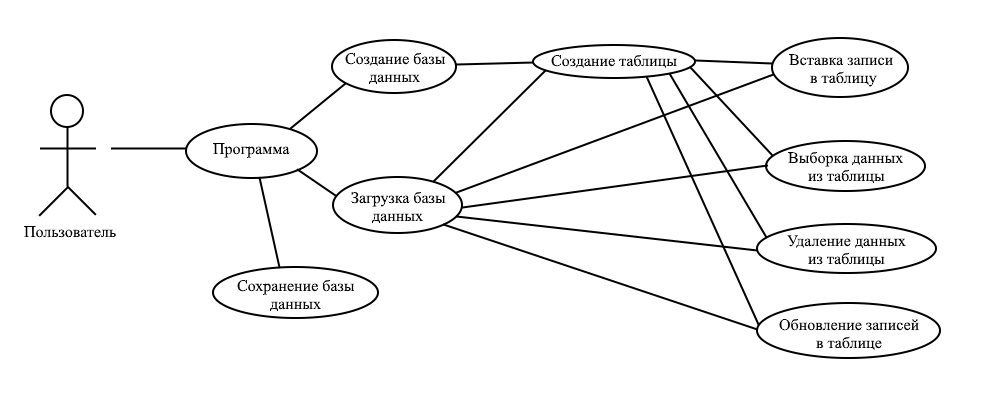
\includegraphics[width=1\linewidth]{images/prec}
	\caption{Диаграмма прецедентов}
	\label{fig:prec}
\end{figure}

\subsubsection{Сценарии прецедентов программы}

\paragraph{Создание базы данных}

Заинтересованные лица и их требования: пользователь желает создать новую базу данных для хранения информации о таблицах, с возможностью дальнейшего сохранения, загрузки и редактирования.

Предусловие: программа запущена, текущая база данных не выбрана или пользователь хочет создать новую.

Постусловие: создана база данных; пользователь может создавать в ней таблицы и добавлять данные.

Основной успешный сценарий:
\begin{enumerate}
	\item Пользователь вводит в поле ввода команду в формате create database <имя базы>.	
	\item Пользователь нажимает на кнопку Run.	
	\item Программа проверяет наличие базы с таким именем в текущем сеансе и на диске:
	\begin{itemize}
		\item если база уже существует и не открыта, выводится предупреждение;	
		\item если открыта другая база данных — запрашивается подтверждение на создание новой.
	\end{itemize}
	\item Если ранее была открыта другая база, она сериализуется и сохраняется, если пользователь подтвердил сохранение.	
	\item Создаётся новая база данных, в которой инициализируются пустой список таблиц и идентификатор имени.	
	\item Созданная база данных устанавливается как текущий рабочий объект.
	\item Выводится сообщение об успешном создании базы данных.	
\end{enumerate}

\paragraph{Создание таблицы}

Заинтересованные лица и их требования: пользователь хочет определить структуру новой таблицы, включающей названия и типы столбцов, в рамках активной базы данных.

Предусловие: открыта и активна база данных, в которой ещё не существует таблицы с заданным именем.

Постусловие: создана таблица с заданными колонками и типами данных и добавлена в базу данных.

Основной успешный сценарий:
\begin{enumerate}
	\item Пользователь вводит в поле ввода команду create table <имя таблицы> <название столбца1> <тип1> <название столбца2> <тип2>... .
	\item Пользователь нажимает на кнопку Run.	
	\item Программа выполняет предварительный разбор команды, разделяя имя таблицы и пары название + тип.	
	\item Программа проверяет:
	\begin{itemize}
		\item корректность имени таблицы;	
		\item уникальность имён столбцов;	
		\item допустимость типов (integer, float, string).
	\end{itemize}
	\item При наличии ошибок система выводит понятное сообщение с подсказкой и отменяет создание.	
	\item При успешной валидации создаётся таблица, в которую записываются:
	\begin{itemize}
		\item список имён столбцов;	
		\item соответствующие типы данных;	
		\item пустой список строк.
	\end{itemize}	
	\item Таблица добавляется в базу данных.	
	\item Выводится сообщение об успешном создании таблицы.
\end{enumerate}

\paragraph{Вставка записи в таблицу}

Заинтересованные лица и их требования: пользователь хочет добавить новую строку данных в выбранную таблицу, соблюдая типы данных, заданные при создании таблицы.

Предусловие: в базе данных должна существовать хотя бы одна таблица. Пользователь знает структуру таблицы и допустимые типы данных.

Постусловие: новая запись добавлена в таблицу, данные сериализуются в оперативной памяти. В случае ошибки типизации — запись не производится.

Основной успешный сценарий:
\begin{enumerate}
	\item Пользователь вводит в поле ввода команду insert into <имя таблицы> values <значение1> <значение2>... .	
	\item Пользователь нажимает на кнопку Run.	
	\item Программа определяет таблицу по имени и извлекает информацию о столбцах и их типах.	
	\item Каждое значение из команды обрабатывается через синтаксический разбор и приводится к нужному типу.	
	\item Программа проверяет:
	\begin{itemize}
		\item соответствие количества значений числу столбцов;	
		\item соответствие типов.
	\end{itemize}
	\item Если проверка не пройдена, отображается окно с ошибкой и описанием проблемы.	
	\item При успешной валидации в таблицу добавляется новая строка с указанными значениями.	
	\item Таблица обновляется в графическом интерфейсе.
\end{enumerate}

\paragraph{Выборка данных из таблицы}

Заинтересованные лица и их требования: пользователь хочет получить данные из таблицы, отфильтрованные по определённым условиям, с выбором конкретных столбцов.

Предусловие: существует хотя бы одна таблица с данными. Пользователь знает названия столбцов и возможные условия фильтрации.

Постусловие: на экране появляется таблица с данными, удовлетворяющими условию и содержащая выбранные столбцы.

Основной успешный сценарий:
\begin{enumerate}
	\item Пользователь вводит в поле ввода команду select <столбец1> <столбец2> ... from <имя таблицы> [where <условие>].
	\item Пользователь нажимает на кнопку Run.	
	\item Программа разбирает команду:
	\begin{itemize}
		\item выделяет список столбцов;		
		\item определяет имя таблицы;		
		\item извлекает и парсит условие (если есть).
	\end{itemize}
	\item Программа извлекает из таблицы данные, удовлетворяющие фильтру.	
	\item Выбираются значения только указанных пользователем столбцов.	
	\item Таблица обновляется в графическом интерфейсе: устанавливаются выбранные заголовки, выводятся строки.	
	\item Если запрос некорректен (неверный синтаксис или ошибка в условии), выводится понятное сообщение об ошибке.
\end{enumerate}

\paragraph{Удаление данных из таблицы}

Заинтересованные лица и их требования: пользователь желает удалить одну или несколько строк таблицы, удовлетворяющих заданному условию.

Предусловие: существует таблица с данными. Пользователь знает структуру данных и условия фильтрации.

Постусловие: из таблицы удалены строки, для которых выполняется условие. Оставшиеся строки остаются без изменений.

Основной успешный сценарий:
\begin{enumerate}
	\item Пользователь вводит в поле ввода команду delete from <имя таблицы> [where <условие>].
	\item Пользователь нажимает на кнопку Run.		
	\item Программа разбирает команду, извлекает имя таблицы и условие (если указано).	
	\item Условие обрабатывается через ast, компилируется в функцию фильтрации.	
	\item Программа проходит по каждой строке таблицы: если условие верно, то строка исключается.	
	\item По завершении удаления данные в таблице обновляются.	
	\item Таблица обновляется в графическом интерфейсе.
\end{enumerate}

\paragraph{Обновление записей в таблице}

Заинтересованные лица и их требования: пользователь желает изменить значения одного или нескольких столбцов для всех строк, удовлетворяющих заданному условию.

Предусловие: существует таблица с данными. Указанные столбцы существуют, новые значения допустимы по типу.

Постусловие: в таблице изменены данные в указанных столбцах для строк, удовлетворяющих условию.

Основной успешный сценарий:
\begin{enumerate}
	\item Пользователь вводит в поле ввода команду update <имя таблицы> set <столбец1> <значение1> ... [where <условие>].
	\item Пользователь нажимает на кнопку Run.		
	\item Программа извлекает имя таблицы, пары столбец + значение и условие (если указано).	
	\item Каждое новое значение разбирается и приводится к типу, заданному для соответствующего столбца.	
	\item Программа применяет условие ко всем строкам: если условие выполняется, то обновляются нужные поля.	
	\item Если хотя бы одно значение имеет несовместимый тип, операция прерывается.	
	\item Данные в таблице обновляются.
	\item Таблица обновляется в графическом интерфейсе.
\end{enumerate}

\paragraph{Сохранение базы данных}

Заинтересованные лица и их требования: пользователь хочет сохранить текущую базу данных с таблицами и данными на диск, чтобы в будущем загрузить её.

Предусловие: выбрана и активна база данных.

Постусловие: файл .db с сериализованным объектом базы сохранён на диск в папке databases/.

Основной успешный сценарий:
\begin{enumerate}
	\item Пользователь выбирает File -> Save из меню.	
	\item Программа проверяет, выбрана ли активная база. Если нет — выводит сообщение об ошибке.	
	\item Используется pickle для сериализации объекта базы в байтовый поток.	
	\item Байты сохраняются в файл databases/<имя базы>.db.	
	\item Программа подтверждает успешное сохранение.
\end{enumerate}

\paragraph{Загрузка базы данных}

Заинтересованные лица и их требования: пользователь хочет загрузить ранее сохранённую базу, чтобы продолжить работу с таблицами.

Предусловие: файл базы данных ранее был сохранён и доступен на диске.

Постусловие: объект базы данных загружен в память, пользователь может выполнять над ним операции.

Основной успешный сценарий:
\begin{enumerate}
	\item Пользователь выбирает File -> Open из меню.	
	\item Открывается диалог выбора файла. Пользователь выбирает .db файл.	
	\item Текущая активная база данных сохраняется в свой файл.
	\item Программа десериализует объект с помощью pickle.	
	\item Загруженный объект становится текущей активной базой.	
\end{enumerate}

\subsection{Требования к оформлению документации}

Разработка программной документации и программного изделия должна производиться согласно ГОСТ 19.102-77 и ГОСТ 34.601-90. Единая система программной документации.

	\section{Технический проект}
\subsection{Общая характеристика организации решения задачи}

Для реализации поставленных задач необходимо спроектировать и разработать программно-информационную систему, включающую в себя реляционную базу данных и приложение с интерфейсом для взаимодействия ней.

\subsection{Обоснование выбора технологии проектирования}

Используемые для создания программно-информационной системы языки и технологии отвечают современным практикам разработки, позволяют достичь высокой производительности и отказоустойчивости программы.

\subsubsection{Язык программирования Python}

В качестве основного языка программирования выбран Python, благодаря его сочетанию выразительности, гибкости и обширной поддержки со стороны сообщества разработчиков. Python — это высокоуровневый, интерпретируемый язык, активно применяющийся как в образовательных, так и в промышленных проектах. Очень широкое применение этот язык нашёл в аналитике данных.

\subsection{Архитектура программной системы}

На рисунке ~\ref{fig:arch} в виде UML-диаграммы представлена архитектура программной системы.
\begin{figure}[H]
	\centering
	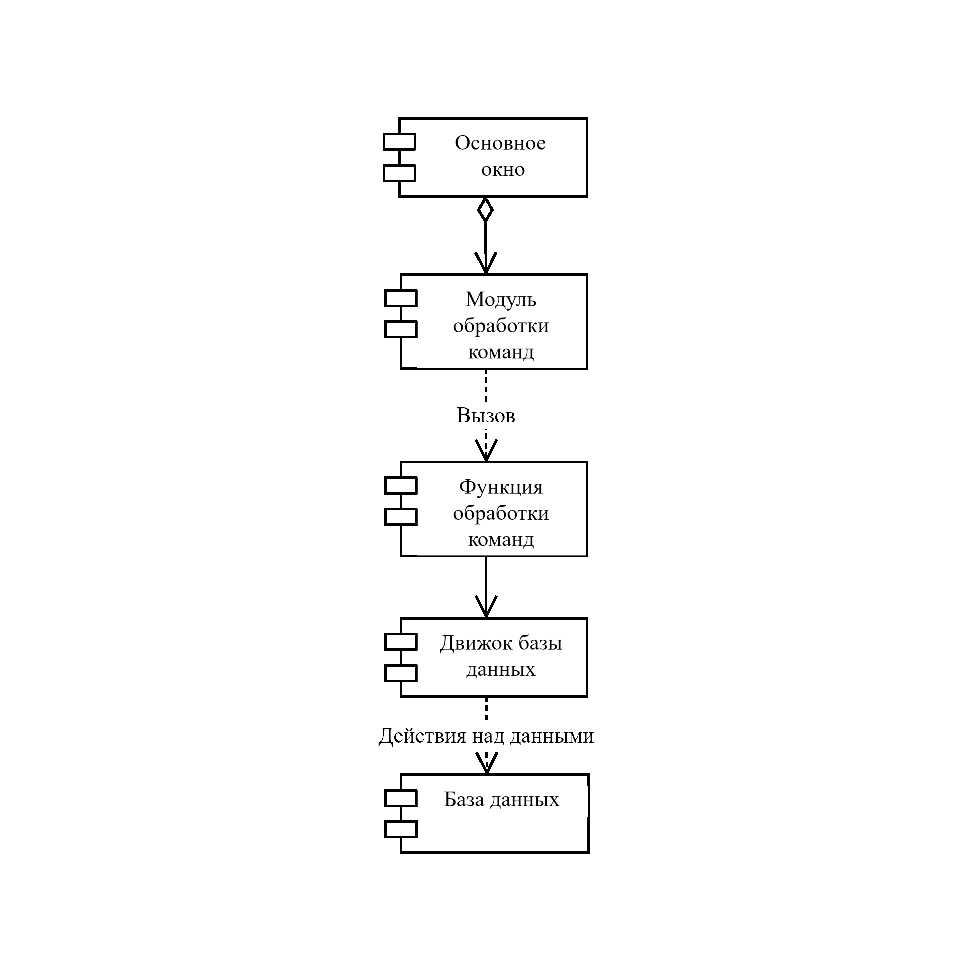
\includegraphics[width=1\linewidth]{images/svg_arch}
	\caption{Архитектура программной системы}
	\label{fig:arch}
\end{figure}

Программа разделена на следующие компоненты:
\begin{enumerate}
	\item Основное окно. Данный модуль реализует интерфейс программной системы.
	\item Модуль обработки команд. Данный модуль обрабатывает пользовательские команды и передаёт соответствующие инструкции в движок базы данных.
	\item Движок базы данных. Этот модуль отвечает за операции над данными в файле базы данных.
	\item Непосредственно сама база данных, представляющая собой .db файл с фиксированной структурой.
\end{enumerate}

\subsection{Архитектура базы данных}

Исходя из требований технического задания, программно-информационная система предназначена для работы с пользовательскими табличными структурами, которые хранятся на диске. Система реализует собственную модель хранения и управления данными средствами языка Python.

\subsubsection{Файл базы данных}

Файл базы данных в реализованной СУБД представляет собой бинарный файл фиксированной структуры, организованный на основе страничного подхода. Такой подход обеспечивает возможность масштабируемого хранения и упрощает работу с диском.

\paragraph{Структура файла}

Файл состоит из трёх основных областей:
\begin{enumerate}
	\item Заголовок файла (3 байта), который содержит информацию о текущем числе таблиц и указатель на первую свободную страницу.
	\item Метаданные таблиц (до 255 таблиц по 4358 байт). Каждая запись содержит название таблицы (до 16 символов); указатели на первую и последнюю страницы таблицы; размер одной записи таблицы в байтах; количество столбцов и описание каждого столбца (название длиной до 16 символов и тип данных).
	\item Страницы хранения данных (по 4096 байт). Каждая страница содержит заголовок (6 байт), содержащий указатель на следующую страницу и количество записей на странице; непосредственно данные -- записи таблицы.
\end{enumerate}

\paragraph{Типы данных}

Поддерживаются три типа данных:
\begin{itemize}
	\item integer -- целочисленный тип, 4 байта;
	\item float -- вещественный тип, 4 байта;
	\item string -- строковый тип, фиксированные 255 байт.
\end{itemize}

\paragraph{Страничная организация}

Каждая страница в файле имеет фиксированный размер в 4096 байт и используется для хранения записей определённой таблицы. Это позволяет организовывать данные в виде цепочек страниц (связный список), где каждая страница знает, какая следующая за ней. Конец списка обозначается специальной константой DEAD\_END, представленной как 0xFFFFFFFF.

Если при вставке записи текущая последняя страница таблицы не имеет достаточно места для новой записи, выделяется новая страница, которая прикрепляется к цепочке.

\subsubsection{Движок базы данных}

Движок базы данных реализует программную логику обработки данных и взаимодействия с бинарным файлом. Он состоит из набора методов класса Database, реализующих основные операции над таблицами и данными: создание таблиц, вставка, выборка, обновление и удаление.

\paragraph{Создание таблицы}

Метод create\_table позволяет создать новую таблицу с заданным именем и структурой. В процессе создания проверяется длина имени таблицы и названий столбцов; генерируется блок метаданных; производится запись в соответствующую область метаданных; выделяется новая страница под таблицу, если необходимо.

\paragraph{Удаление таблицы}

Метод drop\_table позволяет удалить указанную таблицу из базы данных. В процессе удаления полностью стираются все записи таблицы и её метаданные.

Освободившиеся страницы могут использоваться повторно при операциях создания таблиц и вставки данных.

\paragraph{Вставка данных}

Метод insert реализует логику вставки новой записи. Алгоритм включает в себя поиск нужной таблицы по имени; проверку типов данных и количества вставляемых значений; поиск последней страницы таблицы; вставку записи в свободное место либо аллокацию новой страницы при необходимости.

\paragraph{Выборка данных}

Метод select позволяет получить записи таблицы по заданному условию (фильтру). Возвращаются как данные, так и метаинформация о типах столбцов. Алгоритм включает в себя поиск таблицы и считывание метаданных; итерацию по цепочке страниц; распаковку записей и фильтрацию по переданному условию.

\paragraph{Обновление данных}

Метод update позволяет изменить существующие записи. Алгоритм включает в себя поиск таблицы и считывание метаданных; проверка корректности переданных значений; поиск всех записей, удовлетворяющих условию; перезапись выбранных записей на месте в бинарном файле.

\paragraph{Удаление данных}

Метод delete реализует удаление записей. В процессе удаления выполняется выборка всех записей с последующей фильтрацией; оставшиеся записи пакуются заново и перезаписываются в страницы; лишние страницы освобождаются.

Освобождённые после удаления данных страницы могут быть повторно использованы при операциях создания таблиц и вставки данных.

\subsection{Обработчик команд}

Обработчик команд является важным компонентом системы управления базой данных, обеспечивая взаимодействие пользователя с хранилищем данных через текстовые команды. Он интерпретирует пользовательский ввод, распознаёт тип действия и вызывает соответствующие методы движка базы данных. 

\subsubsection{Общий принцип работы}

Обработчик команд реализован в виде функции parse\_command, которая принимает строку с командой и объект базы данных. На первом этапе осуществляется предварительная обработка строки: строка разбивается на токены с использованием метода split(). Первый токен интерпретируется как ключевое слово действия -- create, drop, insert, select, delete или update. В зависимости от распознанного действия вызывается соответствующая логика обработки команды.

\subsubsection{Обработка условий where}

Для разбора логических выражений, указываемых в where-части команд, используется встроенный модуль ast (Abstract Syntax Tree). Это позволяет в качестве условий записывать логические выражения на синтаксисе Python. В условии допускается использование математических операций (+, -, *, /, **), операторов сравнения (>, <, >=, <=, ==, !=) и логических операторов (and, or, not). Выражения обрабатываются функцией eval\_node.

\subsubsection{Синтаксис SQL-команд}

\begin{enumerate}
	\item Создание базы данных: create database <название\_БД>.
	\item Создание таблицы: create table <имя\_таблицы> <столбец1> <тип1> <столбец2> <тип2> ... .
	\item Удаление таблицы: drop table <имя\_таблицы>.
	\item Вставка данных: insert into <имя\_таблицы> values <значение1> <значение2> ... .
	\item Выборка данных: select <столбцы|*> from <имя\_таблицы> [where <условие>].
	\item Удаление данных: delete from <имя\_таблицы> [where <условие>].
	\item Обновление данных: update <имя\_таблицы> set <столбец1> <значение1> ... [where <условие>].	
\end{enumerate}

\subsection{Проектирование пользовательского интерфейса}

На основании требований к пользовательскому интерфейсу, представленных в пункте 2.3.2 технического задания, был разработан графический интерфейс приложения.

На рисунке ~\ref{fig:interface} представлен макет рабочего окна программы. 

\begin{figure}[H]
	\centering
	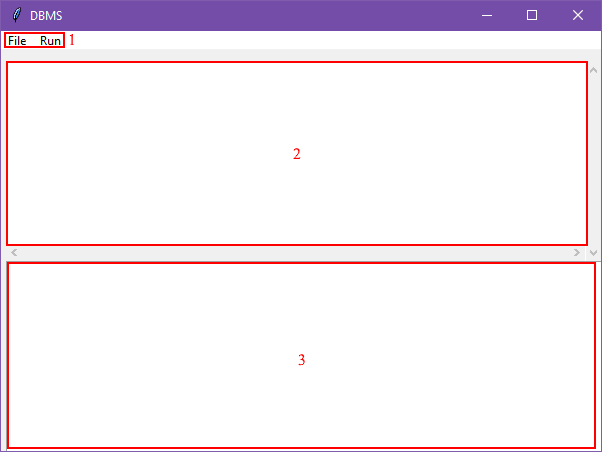
\includegraphics[width=1\linewidth]{images/interface}
	\caption{Макет рабочего окна программы}
	\label{fig:interface}
\end{figure}

Макет содержит следующие элементы:
\begin{enumerate}
	\item Главное меню
	
	Главное меню реализовано на основе виджета tk.Menu и состоит из двух основных разделов:
	\begin{itemize}
		\item Select database -- вызывает окно выбора файла базы данных;
		\item Run -- команда запуска обработки пользовательского ввода, выполняющей анализ текста, введённого в поле SQL-команды, и выполнение соответствующих операций.
	\end{itemize}
	Меню охватывает основные действия, необходимые для работы пользователя с базой данных, и остаётся доступным вне зависимости от текущего состояния приложения.
	
	\item Область отображения таблиц
	
	Эта часть интерфейса занимает верхнюю половину окна и реализована с помощью контейнера tk.Frame и виджета ttk.Treeview, предназначенного для отображения табличных структур в виде древовидной таблицы с колонками. Таблица автоматически подстраивается под содержимое и заполняет всё доступное пространство. Для удобства просмотра добавлены горизонтальная и вертикальная полосы прокрутки.
	
	При проведении операций над данными интерфейс обновляется динамически, подставляя актуальные данные в таблицу.
	
	\item Поле ввода команд
	
	В нижней части окна находится текстовое поле tk.Text, предназначенное для ввода пользователем команд на SQL-подобном языке. Это основная точка взаимодействия между пользователем и программной системой.
	
	По нажатию пункта Run введённая команда передаётся в обработчик команд. Результат выполнения команды отображается либо в таблице, либо во всплывающем сообщении.
\end{enumerate}

	\ifПрактика{}\else{
		\section{Рабочий проект}

\subsection{Спецификация компонентов и классов программы}

\subsubsection{Модуль main.py}

Модуль предоставляет графический интерфейс для управления базами данных. 

Класс модуля -- MainWindow.

Описание класса MainWindow.
Класс предназначен для управления главным окном приложения и передачи пользовательских команд в обработку. Базовый класс -- Tk, стандартный класс библиотеки Tkinter. Интерфейсы: панель меню, позволяющая выбрать файл базы данных для работы и запустить обработку команды; виджет Treeview, отображающий данные выбранной таблицы; виджет Text, куда пользователь вводит команды. Константы отсутствуют. Внутренние поля представлены в таблице~\ref{table:main_widgets}.

\begin{xltabular}{\textwidth}{|X|X|X|}
	\caption{Внутренние поля класса MainWindow\label{table:main_widgets}} \\
	\hline 
	\centrow Внутреннее поле & 
	\centrow Тип & 
	\centrow Описание \\ 
	\hline 
	\endfirsthead
	
	\caption*{Продолжение таблицы \ref{table:main_widgets}} \\
	\hline 
	\centrow Внутреннее поле & 
	\centrow Тип & 
	\centrow Описание \\ 
	\hline 
	\endhead
	
	selected\_db & Database & Активная база данных, над которой проводятся операции \\ \hline
	main\_menu & Menu & Меню, содержащее пункт для выбора базы данных и пункт для запуска команды \\ \hline
	table\_frame & Frame & Фрейм, содержащий в себе табличный виджет Treeview и скроллбары для его прокрутки \\ \hline
	table & Treeview & Виджет для визуального отображения таблиц и выборки данных \\ \hline
	ysb & Scrollbar & Скроллбар для вертикальной прокрутки таблицы \\ \hline
	xsb & Scrollbar & Скроллбар для горизонтальной прокрутки таблицы \\ \hline
	sql\_field\_frame & Frame & Фрейм, содержащий текстовое поле для ввода команд \\ \hline
	sql\_field & Text & Текстовое поле для ввода команд \\ \hline
\end{xltabular}
Методы класса представлены в таблице~\ref{table:main_method}.
\renewcommand{\arraystretch}{0.8} % уменьшение расстояний до сетки таблицы
\begin{xltabular}{\textwidth}{|>{\hsize=0.85\hsize\raggedright\arraybackslash}X|
		>{\hsize=0.85\hsize\setlength{\baselineskip}{0.7\baselineskip}}X|
		>{\hsize=1.0\hsize}X|
		>{\hsize=1.3\hsize}X|}
	\caption{Методы класса MainWindow\label{table:main_method}}\\
	\hline 
	\centrow \setlength{\baselineskip}{0.7\baselineskip} Название метода & 
	\centrow Параметры метода &
	\centrow Возвращаемое значение & 
	\centrow Назначение метода \\ 
	\hline 
	\endfirsthead
	
	\caption*{Продолжение таблицы \ref{table:main_method}}\\
	\hline 
	\centrow Название метода & 
	\centrow Параметры метода &
	\centrow Возвращаемое значение & 
	\centrow Назначение метода \\ 
	\hline 
	\endhead
	
	\_\_init\_\_ & Не имеет & Не имеет  & Инициализирует графический интерфейс приложения, включая его макет и элементы \\ \hline 
	update\_table & headings -- названия столбцов отображаемой таблицы; contents -- содержимое отображаемой таблицы & Не имеет & Обновляет визуальное отображение таблицы в интерфейсе \\ \hline
	select\_database & Не имеет & Не имеет & Вызывает окно для выбора файла базы данных \\ \hline
	execute\_sql & Не имеет & Не имеет & Вызывает функцию обработки команд из модуля parser.py \\ \hline
	
\end{xltabular}
\renewcommand{\arraystretch}{1.0} % восстановление сетки
\vspace{-\baselineskip}

\subsubsection{Модуль parser.py}

Модуль отвечает за обработку пользовательских команд. Не содержит классов и констант. Методы модуля представлены в таблице~\ref{table:parser_method}.
\begin{xltabular}{\textwidth}{|>{\hsize=0.85\hsize\raggedright\arraybackslash}X|
		>{\hsize=0.85\hsize\setlength{\baselineskip}{0.7\baselineskip}}X|
		>{\hsize=1.0\hsize}X|
		>{\hsize=1.3\hsize}X|}
	\caption{Методы модуля parser.py\label{table:parser_method}}\\
	\hline 
	\centrow \setlength{\baselineskip}{0.7\baselineskip} Название метода & 
	\centrow Параметры метода &
	\centrow Возвращаемое значение & 
	\centrow Назначение метода \\ 
	\hline 
	\endfirsthead
	
	\caption*{Продолжение таблицы \ref{table:parser_method}}\\
	\hline 
	\centrow Название метода & 
	\centrow Параметры метода &
	\centrow Возвращаемое значение & 
	\centrow Назначение метода \\ 
	\hline 
	\endhead
	
	eval\_node & node -- условие where; row (значение по умолчанию -- None) -- строка таблицы, из которой нужно взять значения по столбцам & Результат логического выражения в условии where  & Вычисляет значение логического выражения в условии where для переданной строки таблицы \\ \hline 
	parse\_command & command -- команда, введённая пользователем в текстовое поле; db -- движок активной на данный момент базы данных, которому будут передаваться инструкции & Названия столбцов и содержимое для таблицы в интерфейсе & Обрабатывает пользовательские команды и передаёт инструкции для выполнения в движок базы данных \\ \hline	
\end{xltabular}
\renewcommand{\arraystretch}{1.0} % восстановление сетки
\vspace{-\baselineskip}

\subsubsection{Модуль database.py}

Модуль представляет собой движок, реализующий операции над файлом базы данных.

Класс модуля: Database.

Константы модуля представлены в таблице~\ref{table:db_const}.

\renewcommand{\arraystretch}{0.8}
\begin{xltabular}{\textwidth}{|>{\hsize=1.1\hsize\raggedright\arraybackslash}X|>{\hsize=0.95\hsize\raggedright\arraybackslash}X|>{\hsize=0.95\hsize\raggedright\arraybackslash}X|}
	\caption{Константы модуля database.py\label{table:db_const}} \\
	\hline 
	\centrow Имя константы & 
	\centrow Тип & 
	\centrow Описание \\ 
	\hline 
	\endfirsthead
	
	\caption*{Продолжение таблицы \ref{table:db_const}} \\
	\hline 
	\centrow Имя константы & 
	\centrow Тип & 
	\centrow Описание \\ 
	\hline 
	\endhead
	
	TABLE\_META\_SIZE & int & Размер метаданных таблицы в байтах \\ \hline
	MAX\_TABLE\_COUNT & int & Максимально доступное количество таблиц в базе данных \\ \hline
	MAX\_COLUMN\_COUNT & int & Максимально доступное количество столбцов в таблице \\ \hline
	PAGE\_SIZE & int & Размер одной страницы таблицы в байтах \\ \hline
	DATA\_TYPES & dict & Словарь для сопоставления названий типов данных с их индексом в файле БД \\ \hline
	STRUCT\_TYPES & dict & Словарь для сопоставления типов данных с форматом упаковки значений соответствующего типа данных в бинарный формат \\ \hline
	CHECK\_TYPES & dict & Словарь для проверки корректности типов данных передаваемых для записи в таблицу значений \\ \hline
	DEAD\_END & int & Значение, которое указывается в последней странице таблицы \\ \hline
\end{xltabular}
\renewcommand{\arraystretch}{1.0} % восстановление сетки
\vspace{-\baselineskip}

Описание класса Database. Класс предназначен для выполнения операций над файлом базы данных. Не наследуется от других классов. Интерфейсы -- общедоступные методы \_\_init\_\_, create\_table, insert, select, update, delete, drop\_table. Константы отсутствуют. Внутреннее поле класса -- filepath (тип str), оно хранит путь к файлу базы данных. Методы класса представлены в таблице~\ref{table:db_method}.

\renewcommand{\arraystretch}{0.8} % уменьшение расстояний до сетки таблицы
\begin{xltabular}{\textwidth}{|>{\hsize=0.85\hsize\raggedright\arraybackslash}X|
		>{\hsize=0.85\hsize\setlength{\baselineskip}{0.7\baselineskip}}X|
		>{\hsize=1.0\hsize}X|
		>{\hsize=1.3\hsize}X|}
	\caption{Методы класса Database\label{table:db_method}}\\
	\hline 
	\centrow \setlength{\baselineskip}{0.7\baselineskip} Название метода & 
	\centrow Параметры метода &
	\centrow Возвращаемое значение & 
	\centrow Назначение метода \\ 
	\hline 
	\endfirsthead
	
	\caption*{Продолжение таблицы \ref{table:db_method}}\\
	\hline 
	\centrow Название метода & 
	\centrow Параметры метода &
	\centrow Возвращаемое значение & 
	\centrow Назначение метода \\ 
	\hline 
	\endhead
	
	\_\_init\_\_ & path -- путь к файлу БД & Не имеет  & Инициализирует движок для работы с файлом БД по указанному пути, если такого файла нет, то создаёт его \\ \hline 
	\_allocate\_page & Не имеет & Не имеет & Добавляет пустую страницу в файл БД \\ \hline
	create\_table & table\_name -- имя таблицы; columns -- названия столбцов и их типы данных & Не имеет & Создаёт новую таблицу с указанными именем и столбцами \\ \hline
	insert & table\_name -- имя таблицы; values -- значения, которые будут вставлены в таблицу & Не имеет & Добавляет в страницу новую запись с указанными значениями \\ \hline
	select & table\_name -- имя таблицы; columns -- список столбцов для выборки; where (значение по умолчанию -- lambda row: True) -- условие, по которому будет производиться выборка & Названия и типы данных выбранных столбцов; данные, удовлетворяющие условию & Производит выборку данных в указанных столбцах из строк, удовлетворяющих условию \\ \hline
	update & table\_name -- имя таблицы; updated\_values -- новые значения; where (значение по умолчанию -- lambda row: True) -- условие, по которому будет производиться обновление & Не имеет & Обновляет данные в указанных столбцах в строках, удовлетворяющих условию \\ \hline	
	delete & table\_name -- имя таблицы; where (значение по умолчанию -- lambda row: True) -- условие, по которому будет производиться удаление & Не имеет & Удаляет из таблицы все строки, удовлетворяющие условию \\ \hline
	drop\_table & table\_name -- имя таблицы & Не имеет & Удаляет указанную таблицу из базы данных \\ \hline
	
\end{xltabular}
\renewcommand{\arraystretch}{1.0} % восстановление сетки
\vspace{-\baselineskip}

\subsection{Модульное тестирование разработанной программной системы}

Модульный тест для класса Database из модуля database.py представлен в таблице~\ref{table:db_test}.

\renewcommand{\arraystretch}{0.8}
\begin{xltabular}{\textwidth}{|X|X|X|X|}
	\caption{Модульное тестирование класса Database\label{table:db_test}} \\
	\hline
	\centrow Описание теста &
	\centrow Тестируемая функция & 
	\centrow Входные данные & 
	\centrow Ожидаемый результат \\ 
	\hline 
	\endfirsthead
	
	\caption*{Продолжение таблицы \ref{table:db_test}} \\
	\hline 
	\centrow Описание теста & 
	\centrow Тестируемая функция & 
	\centrow Входные данные & 
	\centrow Ожидаемый результат \\ 
	\hline 
	\endhead
	
	Проверка инициализации базы данных & \_\_init\_\_ & Путь к новому файлу &  Файл создан, количество таблиц в созданной БД: 0, индекс свободной страницы: 0 \\ \hline
	Проверка создания таблицы & create\_table & Название и словарь из 3 колонок & Таблица создана, метаданные корректны \\ \hline
	Проверка обработки ошибок при создании таблицы & create\_table & 1. Слишком длинное имя таблицы\newline2. Слишком много колонок\newline3. Слишком длинное имя колонки\newline4. Неизвестный тип данных & Соответствующая ошибка в каждом случае \\ \hline
	Проверка вставки и выборки данных & insert, select & 3 записи в таблицу & Корректное количество и содержимое записей \\ \hline
	Проверка выборки с указанием колонок & select & Названия нужных колонок & Данные только из указанных колонок \\ \hline
	Проверка выборки с фильтром (where) & select & Условие where для выборки & Все записи, соответствующие условию \\ \hline
	Проверка обработки ошибок при вставке & insert & 1. Несуществующая таблица\newline2. Неверное количество значений\newline3. Несоответствие типов & Соответствующая ошибка в каждом случае \\ \hline
	Проверка обновления записей по условию & update & Данные для замены и условие where & Все записи, соответствующие условию, обновлены новыми данными \\ \hline
	Проверка обработки ошибок при обновлении & update & 1. Несуществующая таблица\newline2. Несуществующая колонка\newline3. Несоответствие типов & Соответствующая ошибка в каждом случае \\ \hline
	Проверка удаления данных по условию & delete & Таблица и условие where & Данные удалены в соответствии с условиями \\ \hline
	Проверка удаления таблицы & drop\_table & Таблица с 1 записью & Таблица удалена, обращение к ней вызывает ошибку, количество таблиц в файле: 0 \\ \hline
	Проверка работы с несколькими таблицами & create\_table, insert, select & 2 таблицы с разными данными & Данные в таблицах не пересекаются, операции работают независимо \\ \hline
\end{xltabular}
\renewcommand{\arraystretch}{1.0}
\vspace{-\baselineskip}

Модульный тест для функций eval\_node и parse\_command из модуля parser.py представлен в таблице~\ref{table:parser_test}.

\renewcommand{\arraystretch}{0.8}
\begin{xltabular}{\textwidth}{|X|X|X|X|}
	\caption{Модульное тестирование parser.py\label{table:parser_test}} \\
	\hline
	\centrow Описание теста &
	\centrow Тестируемая функция & 
	\centrow Входные данные & 
	\centrow Ожидаемый результат \\ 
	\hline 
	\endfirsthead
	
	\caption*{Продолжение таблицы \ref{table:parser_test}} \\
	\hline 
	\centrow Описание теста & 
	\centrow Тестируемая функция & 
	\centrow Входные данные & 
	\centrow Ожидаемый результат \\ 
	\hline 
	\endhead
	
	Проверка обработки констант разных типов & eval\_node & Константы разных типов & Значения соответствующих констант \\ \hline
	Проверка доступа к переменным в контексте & eval\_node & Имя переменной и контекст (словарь) & Значение переменной в заданном контексте \\ \hline
	Проверка бинарных операций & eval\_node & Выражения с математическими операторами (+, -, *, /, //, \%, **) & Корректные результаты арифметических операций \\ \hline
	Проверка операторов сравнения & eval\_node & Выражения с операторами сравнения (>, >=, <, <=, ==, !=) & Корректные результаты сравнений \\ \hline
	Проверка логических операторов & eval\_node & and и or с разными комбинациями значений & Корректные результаты логических операций \\ \hline
	Проверка унарных операторов & eval\_node & Унарные операторы (унарный минус, not), применённые к различным значениям & Корректные результаты применения унарных операторов \\ \hline
	Проверка обработки пустой команды & parse\_command & Пустая строка & Ошибка \\ \hline
	Проверка создания таблицы & parse\_command & 1. Корректная команда\newline2. Ошибки синтаксиса & 1. Таблица создана\newline2. Ошибка\\ \hline
	Проверка создания БД & parse\_command & Команда создания БД & Создан файл БД, возвращен объект Database \\ \hline
	Проверка вставки данных & parse\_command & 1. Корректная команда\newline2. Ошибки синтаксиса & 1. Данные добавлены\newline2. Ошибка\\ \hline
	Проверка выборки данных & parse\_command & 1. Корректная команда\newline2. Ошибки синтаксиса & 1. Выбраны корректные данные\newline2. Ошибка\\ \hline
	Проверка обновления данных & parse\_command & 1. Корректная команда\newline2. Ошибки синтаксиса & 1. Данные обновлены\newline2. Ошибка\\ \hline
	Проверка удаления данных & parse\_command & 1. Корректная команда\newline2. Ошибки синтаксиса & 1. Данные удалены\newline2. Ошибка\\ \hline
	Проверка удаления таблицы & parse\_command & 1. Корректная команда\newline2. Ошибки синтаксиса & 1. Таблица удалена, при попытке обращения к ней выдаётся ошибка\newline2. Ошибка\\ \hline
\end{xltabular}
\renewcommand{\arraystretch}{1.0}
\vspace{-\baselineskip}

\subsection{Системное тестирование разработанной программной системы}

Для проведения системного тестирования был использован файл базы данных, содержащий таблицу с сотней записей.

На рисунке~\ref{fig:dbms_window} представлено главное окно СУБД.
\begin{figure}[H]
	\centering
	\includegraphics[width=0.9\linewidth]{"images/окно субд"}
	\caption{Главное окно программы}
	\label{fig:dbms_window}
\end{figure}

На рисунке~\ref{fig:new_db} показана информация о файле новой базы данных, созданной после ввода команды create database new\_database.
\begin{figure}[H]
	\centering
	\includegraphics[width=0.9\linewidth]{"images/новая бд"}
	\caption{Файл новой базы данных}
	\label{fig:new_db}
\end{figure}

На рисунке~\ref{fig:select} представлено окно выбора файла после нажатия на пункт меню <<Выбрать БД>>.
\begin{figure}[H]
	\centering
	\includegraphics[width=0.9\linewidth]{"images/выбор файла"}
	\caption{Окно выбора файла}
	\label{fig:select}
\end{figure}

На рисунке~\ref{fig:select_sql} представлен результат выборки данных из таблицы.
\begin{figure}[H]
	\centering
	\includegraphics[width=0.9\linewidth]{"images/выборка"}
	\caption{Результат выборки}
	\label{fig:select_sql}
\end{figure}

На рисунке~\ref{fig:insert_sql} представлен результат вставки данных в таблицу.
\begin{figure}[H]
	\centering
	\includegraphics[width=0.9\linewidth]{"images/вставка"}
	\caption{Результат вставки}
	\label{fig:insert_sql}
\end{figure}

На рисунке~\ref{fig:update_sql} представлен результат обновления данных в таблице.
\begin{figure}[H]
	\centering
	\includegraphics[width=0.9\linewidth]{"images/обновление"}
	\caption{Результат обновления}
	\label{fig:update_sql}
\end{figure}

На рисунке~\ref{fig:delete_sql} представлен результат удаления данных из таблицы.
\begin{figure}[H]
	\centering
	\includegraphics[width=0.9\linewidth]{"images/удаление"}
	\caption{Результат удаления}
	\label{fig:delete_sql}
\end{figure}

На рисунке~\ref{fig:error} представлено сообщение об ошибке при неправильно введённой команде выборки.
\begin{figure}[H]
	\centering
	\includegraphics[width=0.7\linewidth]{"images/ошибка"}
	\caption{Ошибка в команде выборки}
	\label{fig:error}
\end{figure}

На рисунке~\ref{fig:error_insert} представлено сообщение об ошибке при неправильно введённой команде вставки.
\begin{figure}[H]
	\centering
	\includegraphics[width=0.7\linewidth]{"images/ошибка вставки"}
	\caption{Ошибка в команде вставки}
	\label{fig:error_insert}
\end{figure}

На рисунке~\ref{fig:error_update} представлено сообщение об ошибке при неправильно введённой команде обновления.
\begin{figure}[H]
	\centering
	\includegraphics[width=0.7\linewidth]{"images/ошибка обновления"}
	\caption{Ошибка в команде обновления}
	\label{fig:error_update}
\end{figure}

На рисунке~\ref{fig:error_delete} представлено сообщение об ошибке при неправильно введённой команде удаления.
\begin{figure}[H]
	\centering
	\includegraphics[width=0.7\linewidth]{"images/ошибка удаления"}
	\caption{Ошибка в команде удаления}
	\label{fig:error_delete}
\end{figure}

На рисунке~\ref{fig:error_table} представлено сообщение об ошибке при попытке обращения к несуществующей таблице.
\begin{figure}[H]
	\centering
	\includegraphics[width=0.7\linewidth]{"images/ошибка таблица"}
	\caption{Обращение к несуществующей таблице}
	\label{fig:error_table}
\end{figure}



\subsection{Сборка программной системы}

Программные компоненты представляют собой файлы исходных кодов программной системы.

Для сборки и компиляции программной системы использовалась библиотека Pyinstaller, позволяющая упаковать все необходимые файлы в один исполняемый файл формата .exe. Данный файл может быть запущен без предварительной установки.

Интерпретация исходных кодов на языке Python выполняется встроенным в исполняемый файл интерпретатором языка и не требует отдельной установки интерпретатора и библиотек на целевую систему.

Все программные компоненты собраны в один исполняемый файл, готовый к запуску в среде Windows.
		\section*{ЗАКЛЮЧЕНИЕ}
\addcontentsline{toc}{section}{ЗАКЛЮЧЕНИЕ}

Развитие информационных технологий и рост объемов данных способствовали повышенному интересу к созданию и совершенствованию систем управления базами данных. Базы данных стали неотъемлемой частью практически всех сфер человеческой деятельности — от бизнеса и государственного управления до научных исследований и повседневной жизни. Умение организовывать, хранить и обрабатывать информацию в структурированной форме имеет решающее значение для повышения эффективности процессов и принятия обоснованных решений.

В условиях возрастающих требований к гибкости, простоте и автономности обработки данных разработка собственных, легковесных и адаптируемых СУБД приобретает всё большую актуальность.

В рамках данной выпускной квалификационной работы была разработана собственная система управления базами данных реляционной модели, реализующая базовые функции создания, хранения, изменения и выборки данных.

Основные результаты работы:

\begin{enumerate}
\item Проведен анализ предметной области. Проведено исследование причин разработки баз данных, областей их применения и перспектив их развития.
\item Разработана концептуальная модель программной системы, определены основные требования к системе и структуре базы данных.
\item Осуществлено проектирование программной системы. Разработана архитектура настольного приложения и базы данных. Разработан пользовательский интерфейс приложения.
\item Реализована программная система, проведено модульное и системное тестирование СУБД.
\end{enumerate}

Все требования, объявленные в техническом задании, были полностью реализованы. Все задачи, поставленные в начале разработки проекта, были решены.

Готовый рабочий проект представлен в виде настольного приложения с графическим интерфейсом.

	}\fi
	\addcontentsline{toc}{section}{СПИСОК ИСПОЛЬЗОВАННЫХ ИСТОЧНИКОВ}

\begin{thebibliography}{9}

    \bibitem{} Кореньков В. В., Иванцова О. В., Филозова И. А. Технологии баз данных. Проектирование реляционных баз данных. – 2022. – Текст~: непосредственный.
    \bibitem{} Осипов Д. Технологии проектирования баз данных. – 2022. – Текст~: непосредственный.
    \bibitem{} Илюшечкин В. Основы использования и проектирования баз данных. Учебник для академического бакалавриата. – 2021. – Текст~: непосредственный.
    \bibitem{} Жидченко Т. В. Базы данных. – 2021. – Текст~: непосредственный.
	\bibitem{} Стасышин В. М. Разработка информационных систем и баз данных. – 2020. – Текст~: непосредственный.
	\bibitem{} Волхонский А. Н. Модели данных при проектировании баз данных автоматизированных систем //Международный студенческий научный вестник. – 2021. – №. 6. – С. 38. – Текст~: непосредственный.
	\bibitem{} Годин В. В., Стружкин Н. П. Базы данных: проектирование. – 2019. – Текст~: непосредственный.
	\bibitem{} Лазицкас Е. А., Загумённикова И. Н., Гилевский П. Г. Базы данных и системы управления базами данных. – 2016. – Текст~: непосредственный.
	\bibitem{} Махкамов Ш. Теоретические основы базы данных (мб) и системы управления базами данных (мббт) //Информатика и инженерные технологии. – 2023. – Т. 1. – №. 1. – С. 90-94. – Текст~: непосредственный.    
	\bibitem{} Тораев М. Ш. Основы реляционных баз данных //КОНЦЕПЦИИ УСТОЙЧИВОГО РАЗВИТИЯ НАУКИ В СОВРЕМЕННЫХ УСЛОВИЯХ. – 2018. – С. 208-210. – Текст~: непосредственный.    
	
\end{thebibliography}

	\ifВКР{\appendix{Представление графического материала}

Графический материал, выполненный на отдельных листах,
изображен на рисунках А.1--А.\arabic{числоПлакатов}.
\setcounter{числоПлакатов}{0}

\renewcommand{\thefigure}{А.\arabic{figure}} % шаблон номера для плакатов

\begin{landscape}

\begin{плакат}
    \includegraphics[width=0.82\linewidth]{Ramka.eps}
    \заголовок{Сведения о ВКРБ}
    \label{pl1:image}      
\end{плакат}

\begin{плакат}
    \includegraphics[width=0.82\linewidth]{plakat2.eps}
    \заголовок{Цель и задачи разработки}
    \label{pl2:image}      
\end{плакат}

\begin{плакат}
	\includegraphics[width=0.82\linewidth]{plakat3.eps}
	\заголовок{Понятие базы данных}
	\label{pl3:image}      
\end{плакат}

\begin{плакат}
	\includegraphics[width=0.82\linewidth]{plakat4.eps}
	\заголовок{СУБД}
	\label{pl4:image}      
\end{плакат}

\begin{плакат}
	\includegraphics[width=0.82\linewidth]{plakat5.eps}
	\заголовок{Классификация СУБД}
	\label{pl5:image}      
\end{плакат}

\begin{плакат}
	\includegraphics[width=0.82\linewidth]{plakat6.eps}
	\заголовок{История развития}
	\label{pl6:image}      
\end{плакат}

\begin{плакат}
	\includegraphics[width=0.82\linewidth]{plakat7.eps}
	\заголовок{Диаграмма прецедентов}
	\label{pl7:image}      
\end{плакат}

\begin{плакат}
	\includegraphics[width=0.82\linewidth]{plakat8.eps}
	\заголовок{Архитектура программной системы}
	\label{pl8:image}      
\end{плакат}

\begin{плакат}
	\includegraphics[width=0.82\linewidth]{plakat9.eps}
	\заголовок{Структура файла БД}
	\label{pl9:image}      
\end{плакат}

\begin{плакат}
	\includegraphics[width=0.82\linewidth]{plakat10.eps}
	\заголовок{Синтаксис SQL-команд}
	\label{pl10:image}      
\end{плакат}

\begin{плакат}
	\includegraphics[width=0.82\linewidth]{plakat11.eps}
	\заголовок{Главное окно программы}
	\label{pl11:image}      
\end{плакат}

\begin{плакат}
	\includegraphics[width=0.82\linewidth]{plakat12.eps}
	\заголовок{Пример использования программы}
	\label{pl12:image}      
\end{плакат}

\begin{плакат}
	\includegraphics[width=0.82\linewidth]{plakat13.eps}
	\заголовок{Заключение}
	\label{pl13:image}      
\end{плакат}


\end{landscape}
}\fi
	\ifПрактика{}\else{\appendix{Фрагменты исходного кода программы}

main.tex
\lstinputlisting[language=Tex, frame=none]{main.tex}

ТехПроект.tex
\lstinputlisting[language=Tex, frame=none]{ТехПроект.tex}

\ifВКР{
\newpage
\addcontentsline{toc}{section}{На отдельных листах (CD-RW в прикрепленном конверте)}
\noindent
\begin{tabular}{p{5.8cm}C{4.8cm}C{4.8cm}}
   Автор ВКР & \lhrulefill{\fill} & \fillcenter\Автор \\
            \setarstrut{\footnotesize}
           & \footnotesize{(подпись, дата)} & \\
            \restorearstrut
   Руководитель ВКР & \lhrulefill{\fill} & \fillcenter\Руководитель \\
            \setarstrut{\footnotesize}
           & \footnotesize{(подпись, дата)} & \\
            \restorearstrut
   Нормоконтроль & \lhrulefill{\fill} & \fillcenter\Нормоконтроль \\
            \setarstrut{\footnotesize}
           & \footnotesize{(подпись, дата)} & \\
            \restorearstrut
\end{tabular}
\vskip 2cm
\begin{center}
\textbf{Место для диска}
\end{center}
}\fi
}\fi
\end{document}
